\documentclass[platz]{tudphygp}
\usepackage{tudphymd,mhchem}

\versuch{Substanzen im Magnetfeld}{SM}

\begin{document}
\maketitle

\section*{Aufgabenstellung} 
\begin{enumerate}
 \item Im inhomogenen Magnetfeld ist nach Gouy die Suszeptibilit�t einer diamagmetischen Substanz (Cu) zu bestimmen.
 \item Mit der Steigh�henmethode wird die paramagnetische Suszeptibilit�t $\chi$ sowie die molare Suszeptibilit�t $\chi_{mol}$ einer 
 $\text{Mn}^{2+}$-L�sung bestimmt.
 \item Berechnung des atomaren magnetischen Moments $\mu'$ eines Mangan-Ions $\text{Mn}^{2+}$.
\end{enumerate}

\section*{Hinweise}
Der Haupt-(Druck)-Schalter befindet sich links neben der T�r. Mit den Zahlen (1,2,3) ist jedem Wei�schen Elektromagneten ein 
Stromversorgungsger�t zugeordnet, das nur eingeschaltet werden kann, wenn hinreichend K�hlwasser flie�t. Bitte langsam hoch-
und runterregeln und niemals Str�me schalten! W�hrend des Messvorgangs m�ssen die Distanzst�cke aus Messing (jeweils $\SI{15}{mm}$) 
an geeigneter Stelle im Luftspalt eingeklemmt sein. Maximale Messzeit: $\SI{20}{min}$, danach K�hlpause. Die Kalibrierungskurven 
$B_L=B_L(I)$ liegen vor.
\begin{description}
\item[1. Versuchsteil:] Zylindermethode nach Gouy
 \begin{itemize}
  \item Nach Bestimmung seiner Abmessungen wird der Kupferzylinder eingeh�ngt und nach Beruhigung die elektrische Waage auf Null 
  abgeglichen. Die Feldst�rke wird zweimal schrittweise hoch und runter geregelt und die zugeh�rigen Masse-Werte werden notiert. 
  Auswertung nach geeigneter Auftragung.
 \end{itemize}
 \item[2. Versuchsteil:] Steigh�henmethode nach Quincke
 \begin{itemize}
  \item F�r die $\text{Mn}^{2+}$-L�sung wird die Dichte berechnet.
  \item F�r die $\text{Mn}^{2+}$-L�sung wird die Feldabh�ngigkeit der Steigh�he (2 mal steigend und fallend) bestimmt.
  \item Aus dem Anstieg der grafischen Darstellung wird $\chi$ ermittelt.
  \item Damit wird zun�chst die Konzentration $n$ kontrolliert. Weiterhin sind die Curiekonstante $C$ und bei bekanntem $n$ das 
  atomare magnetische Moment der $\text{Mn}^{2+}$-Ionen $\mu'=p_{eff}\mu_B$ sowie $p_{eff}$ abzusch�tzen. Wegen
  \begin{equation*}
   \chi=\frac{J}{\mu_0H}=\frac{1}{\mu_0H}\cdot\frac{J_S\mu_0\mu'H}{3kT}=\frac{\mu_0np_{eff}^2\mu_b^2}{3kT}=\frac{C}{T}
  \end{equation*}
  gilt
  \begin{equation*}
    p_{eff}^2=\displaystyle\frac{\chi}{nK^*}\quad\text{mit}\quad K^*=\displaystyle\frac{\mu_0\mu_B^2}{3kT}=\SI{890e-35}{m^3}\quad
    \text{f�r}\quad T=\SI{293}{K}  
  \end{equation*}
  \item Der Neigungswinkel der R�hrchen betr�gt $\alpha=30^\circ$.
  \item Relative Atommassen: $^1\text H$, $^{16}\text O$, $^{\num{35,4}}\text {Cl}$, $^{55}\text{Mn}$
 \end{itemize}
\end{description}

\begin{figure}
\centering
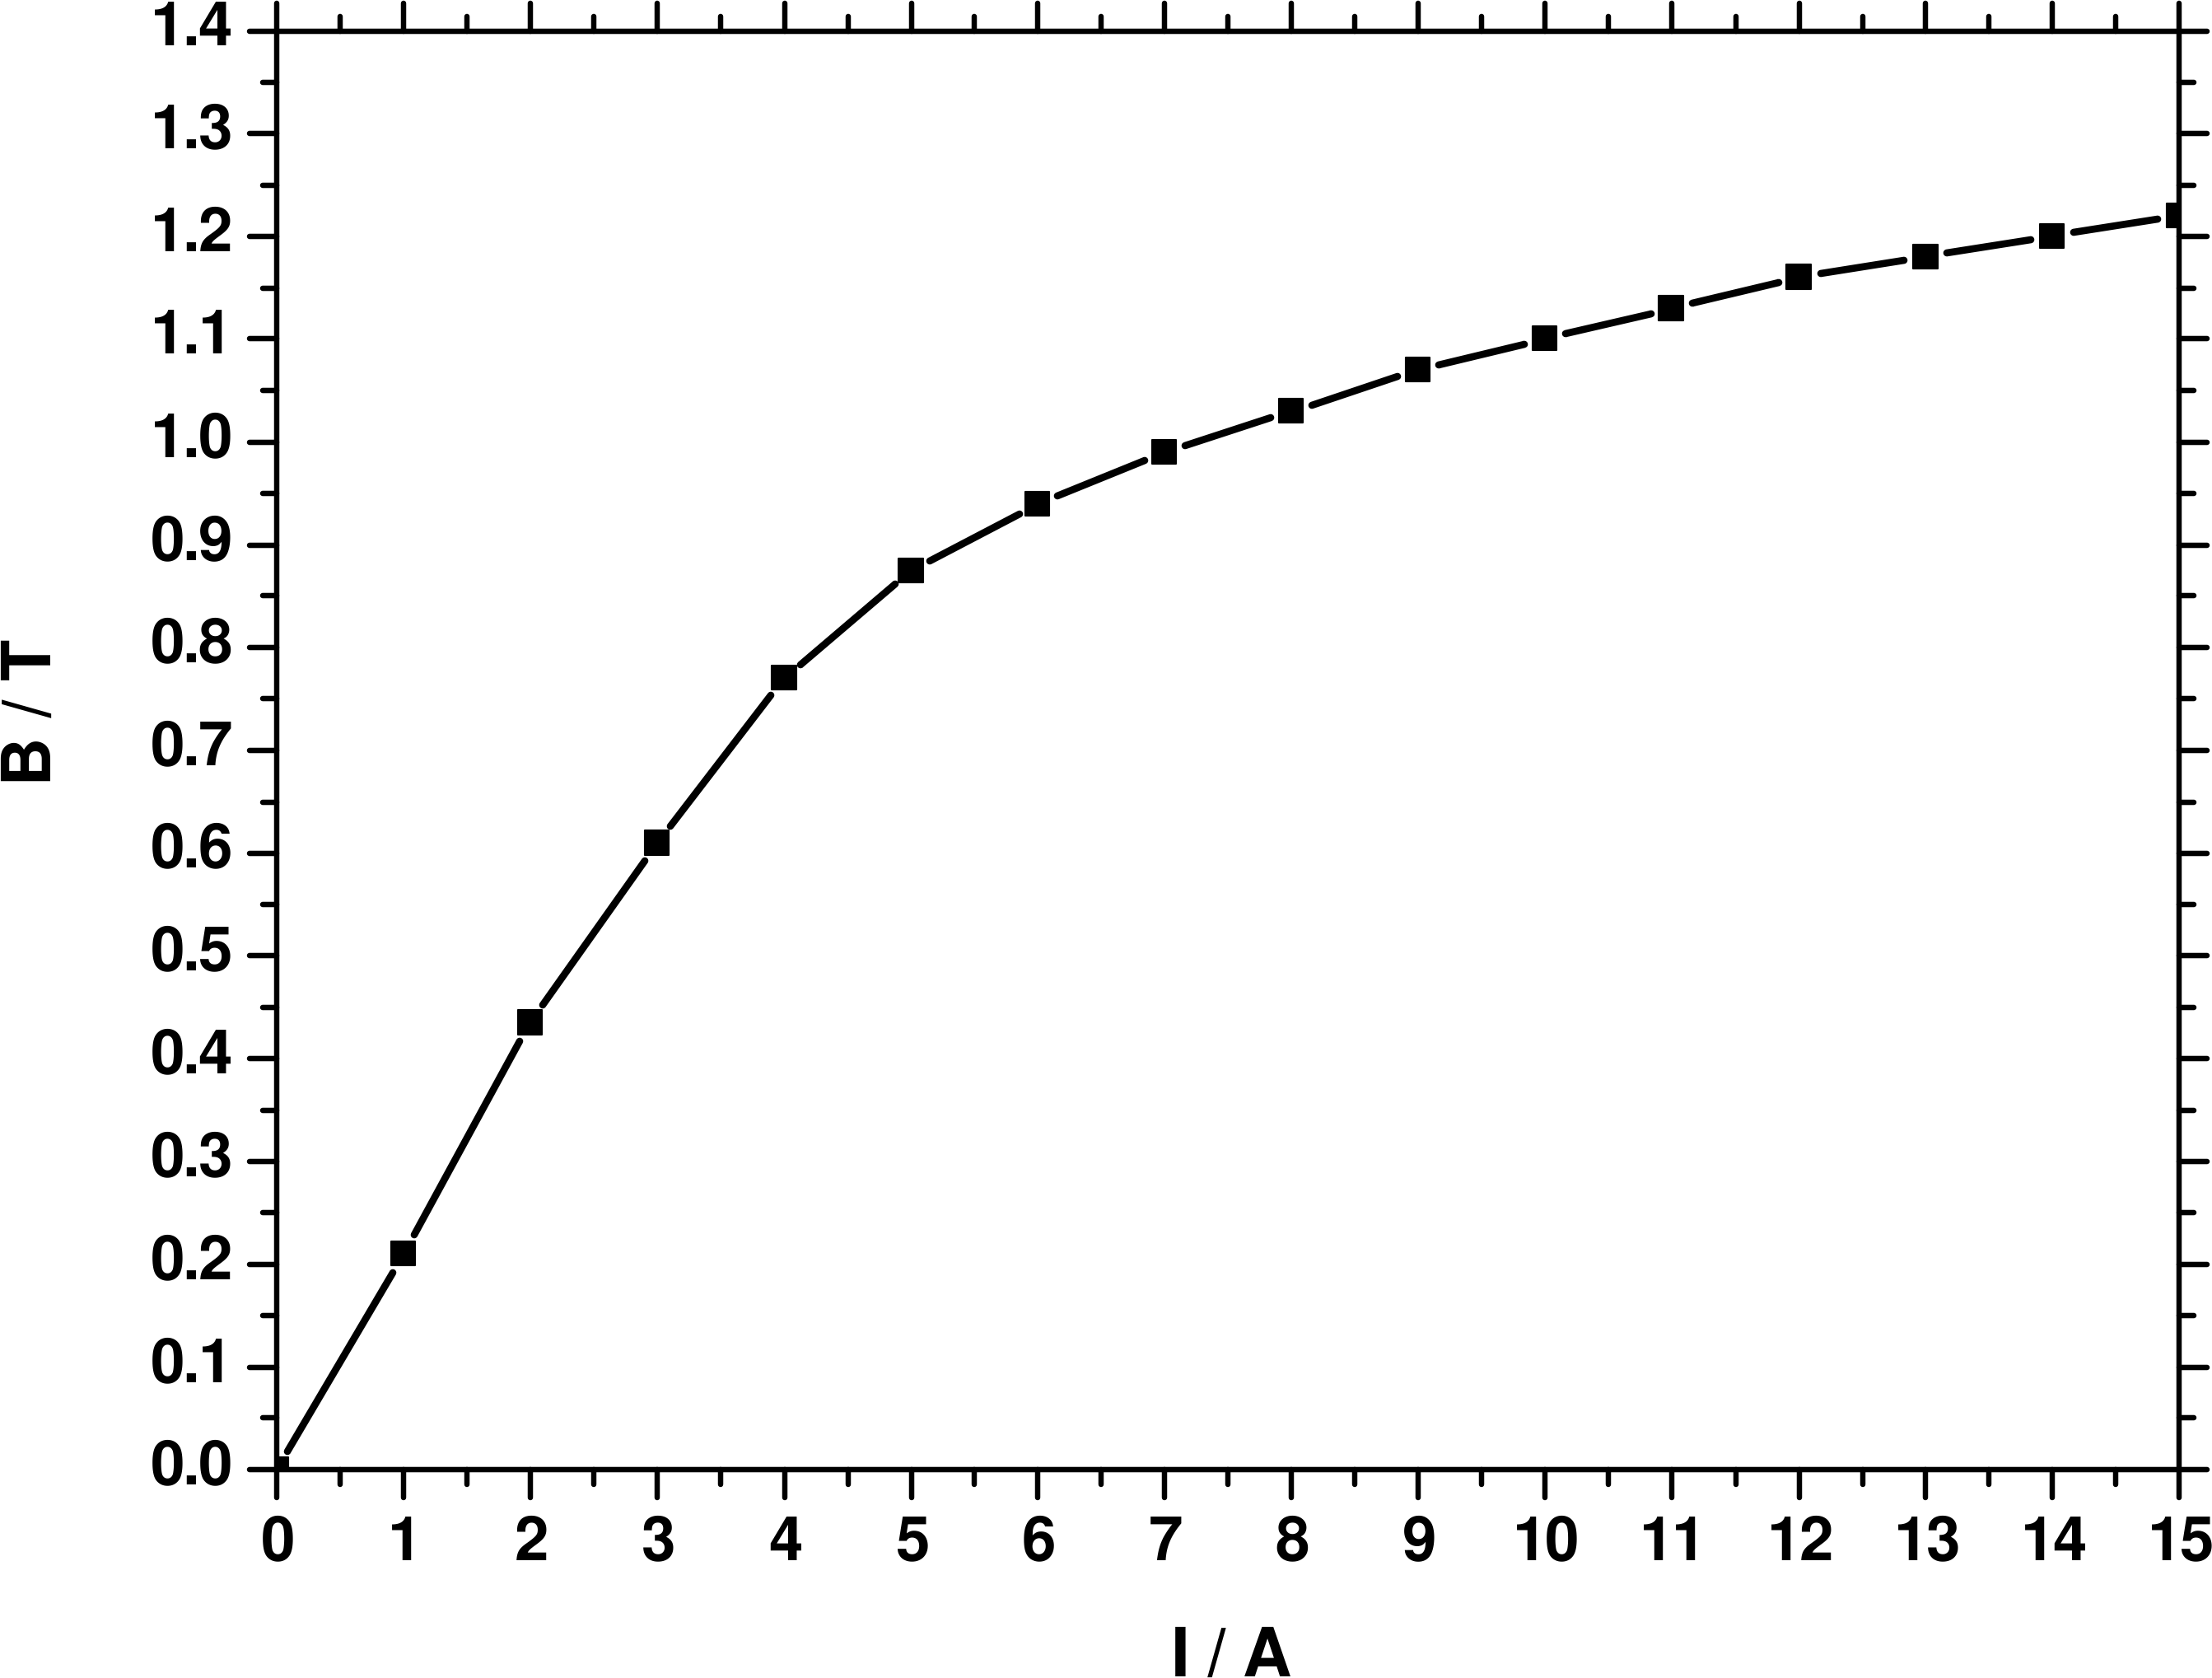
\includegraphics[width=0.7\textwidth]{platz2.png}
\caption{$B(I)$-Zusammenhang f�r den Magneten 2: Polschuhe plan, Abstand $\SI{15}{mm}$, Durchmesser $\SI{100}{mm}$, gemessen in 
Mittelposition homogenes Feld $\pm\SI{40}{mm}$ ($B$, $I$-Fehler $\SI{2,5}{\%}$)}
\end{figure}

\begin{figure}
\centering
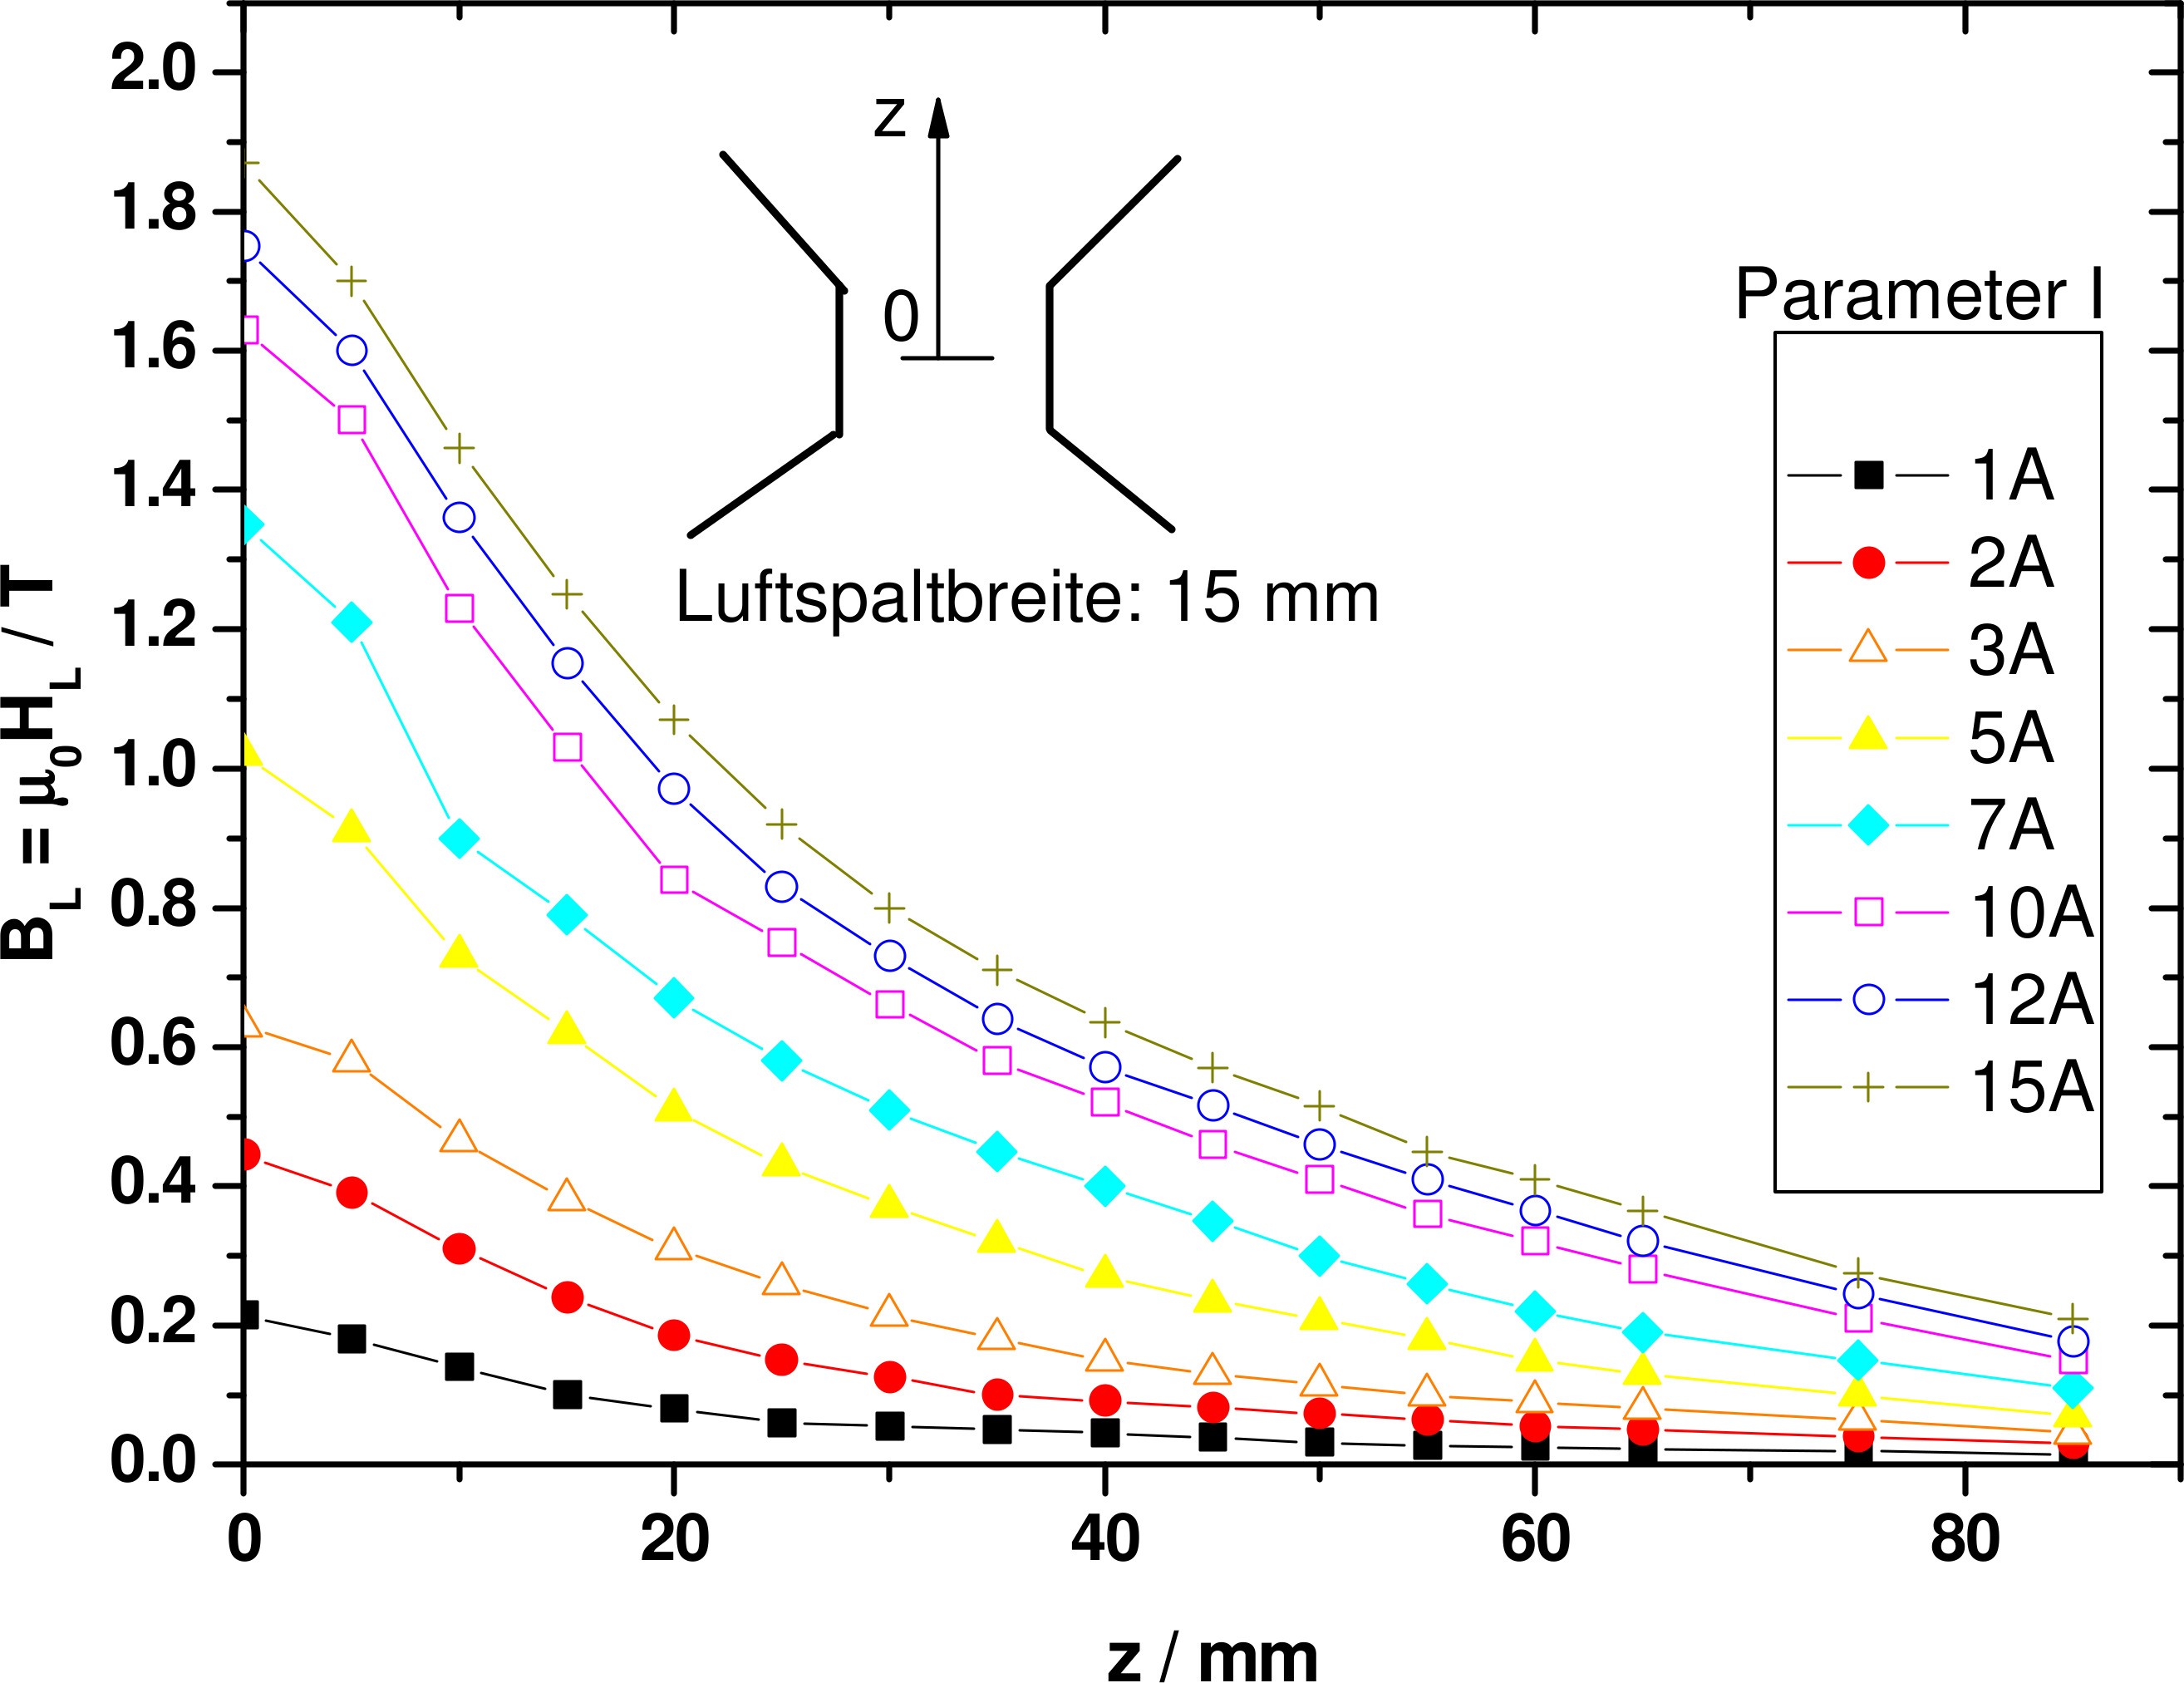
\includegraphics[width=0.7\textwidth]{platz3.png}
\caption{$B(z)$-Zusammenhang f�r den Magneten 3}
\end{figure}
\end{document}
